\chapter{Introduction}
\label{chp:intro}



\section{Definition}
\label{chp:intro:sec:definition}

IT-Security is a generic term for a lot of different topics. Mobile security is a particular part of security with the same concerns but with focus on mobile devices. The rising of mobile devices started with the first mobile phones and handhelds. With arriving the first touchscreen devices and a much higher usability the number of mobile devices rised to a smartphone-penetration of 66\% in 2018. \cite{smartphone-penetration}

\begin{figure}[h]
	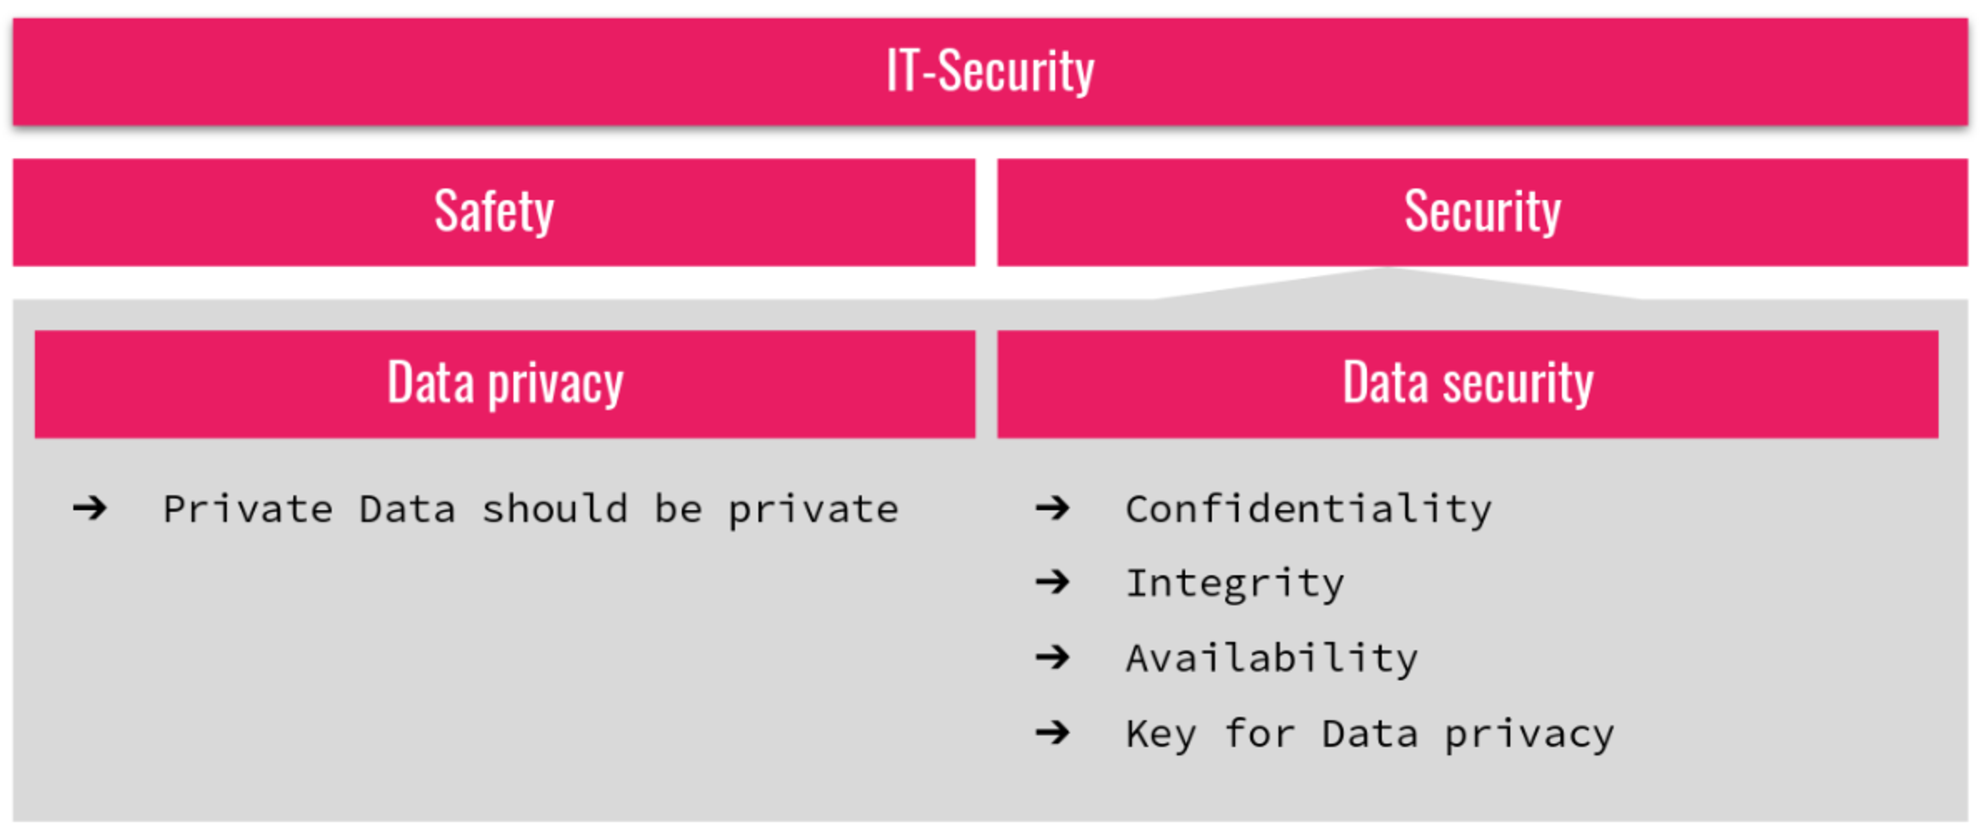
\includegraphics[width=\textwidth, angle=0]{img/it_security.pdf}
		\caption{Parts of IT-Security}
	\label{img:part_it_security}
\end{figure}

\subsection{Safety}
\label{chp:intro:sec:definition:ssec:safety}

The main question in safety is: \textit{Does my application what it is supposed to do?}. \\
So it is about functionality and often directly defined by customers or stakeholder. One strategy to avoid problems with safety topics are automated test. For example unit tests and integration test running by a continuous integration (CI). \\
But safety is not the focused topic.

\subsection{Security}
\label{chp:intro:sec:definition:ssec:safety}

Security is about information and data. Like in Fig. \ref{img:part_it_security} it can be split into privacy and security.

\subsubsection{Privacy}
\label{chp:intro:sec:definition:ssec:safety::sss:privacy}

Privacy' subject is to make sure that personal data like age, name or address are accessible only by people who are allowed. \\
Since \hyperref[https://gdpr-info.eu/]{GDPR} came into force, it is not only a ideological question it is also a lawful question. And not fulfill this law can result in very high fines.\\ The goals, to keep private data private, can only get achieved with security. 

\subsubsection{Security}
\label{chp:intro:sec:definition:ssec:safety::sss:security}

Security has three general targets.

\begin{description}
	\item[Confidentiality] is about making sure to restricted the access to a level where only people with the necessary privileges are allowed to see, change or delete these data.
	
	\item[Integrity] makes sure that every unauthorized change can be detected and changes are verifiable.
	
	\item[Availability] Means that the information should be always available to the user.
\end{description} 

But there are also some more specific target. These does not fit in every use case.

\begin{description}
	\item[Authenticity] aims on reliability. It should be clear that a message comes from the specific sender.
	
	\item[Anonymity] In some cases it should not be possible to connect a network package to a specific person.
\end{description} 

In a lot of cases it is a trade of between these targets. In this case it should be clear why and what it means to not fulfill the target to 100\%.

\newpage
\section{Motivation}
\label{chp:intro:sec:motivation}

Mobile devices get used for a lot of topics. Manage contact, doing phone calls and messaging are only the simplest examples. Nowadays the smartphone is used for nearly everything and became a personal assistant. That means a lot of personal data are stored on the device. Just to mention some of these data:

\begin{itemize}
	\item Identities, for social media but also for credit/customer cards or online banking.
	\item Histories, like browser history or location history
	\item Payments
	\item Location
\end{itemize}

Implementing secure mobile applications can be more difficult than for a regular desktop environment because the user wants a simpler UI and an easy and fast access to their data. So it should be avoided to ask for long inputs or complicated authentication methods.\\
\\
A further difference to the desktop environment is the mobility of these devices. Because of that an smartphone can easily get in the wrong hands. And the connectivity of these devices is higher since they support nearly every modern interface, which can be wired but in the most time is wireless. All these interfaces open a new attack vector, which can be used to get some data or control over the device.\\
\\
But away from the technical background there are more reasons to secure a mobile application. \\
\begin{itemize}
	\item The store provider check their apps for common bugs which can lead to secure gap
	\item Laws like \textit{GDPR} force us to secure user data
	\item Corrupt data inside the app can destroy the user experience
	\item Loosing data can lead to reputational damage
	\item A exploited security issue can cost a lot of money
	\item Your own standards
\end{itemize}


